En esta secci\'on, presentaremos los resultados obtenidos en los experimentos
utilizando lo definido en la secci\'on de desarrollo.

Se buscaron analizar en cada fuente tres tipos de redes segun su escala, es
decir redes pequeña, mediana y gran escala. Estas redes fueron
una hogareña, de unas oficinas, de un laboratorio de una Universidad.

En cada captura se almaceno todo los paquetes que se transmitieron por la red
con el sniffer desarollado como se menciono previamente. Luego analizados
automaticamente por el otro programa `analy\_data` para producir los graficos
que se presentan a continuación.

\subsection{Nodos distinguidos}

En cada experimento se analizaron las dos fuentes de información y se definió
un criterio para distinguir un nodo de cada red. Este criterio consta en que
será distinguido el símbolo con mas probabilidad de ocurrir o equivalentemente
el símbolo que tenga menor información.

Para la fuente $S_2$ una de las hipótesis es que estos nodos "distinguidos" son
nodos especiales como routers, access points, etc. dado que estos participan
en la mayor parte de las comunicaciones con la red como con el exterior.
Por lo cual esto nos daría un método (no 100\% confiable debido a casos
atípicos) de determinar los router en una red.

Otra de las hipótesis que se presenta es que una red \textit{cableada} será
mas "compresible" que una \textit{wireless}. Para esto se mostraron el
cociente de la $\frac{H(S)}{H_{MAX}(S)}$ como se desarrollo en TODO: CITA
y se los comparo entre el mismo tipo de fuente de los distintos experimentos.

\subsection{Descripción de los Gráficos}

En cada experimentación se generaron tres tipos de resultados/gráficos.

\begin{itemize}
	\item Un gráfico que muestra una representación tipo torta de la fuente,
	esto es, la probabilidad de ocurrencia de cada símbolo.  \item Un gráfico
	tipo histograma que muestra para cada símbolo la información de este. Este
	gráfico cuenta además con una barra horizontal que muestra donde se sitúa
	la Entropía de la fuente (en color naranja) y otra barra similar que
	muestra donde se sitúa la Entropía máxima que podría tener la fuente.
	\item Un gráfico con la topología de los mensajes de la red. Donde los
	nodos son \textbf{MAC} address y las aristas representan un paquete de un
	nodo a otro
\end{itemize}

\subsection{Red hogareña}

\subsubsection{Fuente Unicast-Multicast}

 Lo siguiente corresponde a la experimentación realizada para la fuente Unicast-Multicast en una red WiFi domestica.
 
\begin{figure}
	\begin{minipage}[b]{0.9\linewidth}
		\subfloat[Probabilidades de los simbolos de la fuente $S_1$ para la red de hogareña]{
		 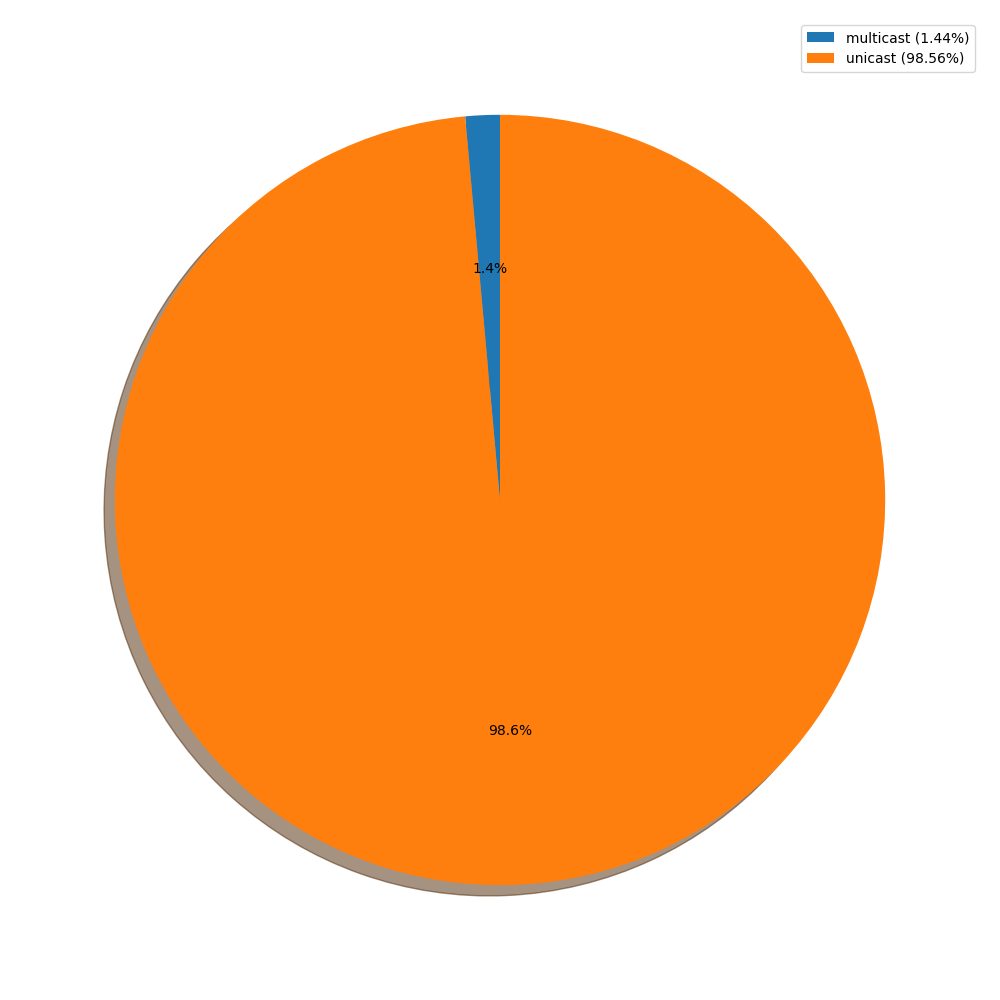
\includegraphics[width=0.45\linewidth]{../plots/mauro_s1_probabilidades.png}
		}
		\subfloat[Información de los simbolos de la fuente $S_1$ para la red de hogareña]{
		 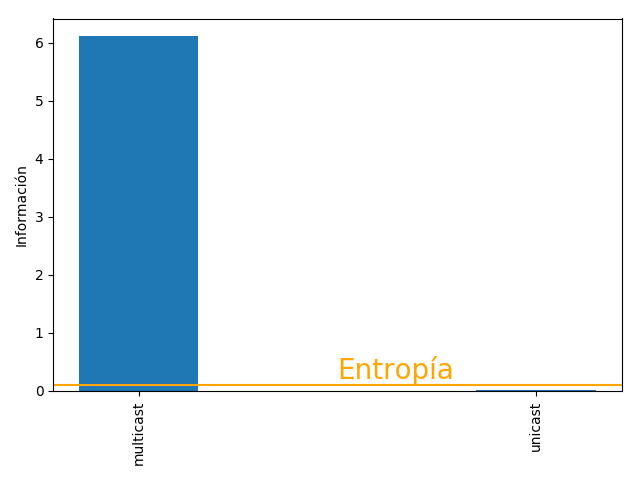
\includegraphics[width=0.55\linewidth]{../plots/mauro_s1_informacion.png}
		}
	\end{minipage}
\end{figure}

Como podemos ver los resultados obtenidos muestran una alta concentración de
paquetes \textit{multicast} por sobre los \textit{unicast}. En consecuencia la
entropía cae abruptamente, ya que como explicamos ésta se maximiza cuando la
distribución de las probabilidades de cada símbolo es equitativa, y baja a
medida que nos alejamos de ello. Nuestra primera impresión era que los
paquetes \textit{unicast} iban a predominar en la captura, sin embargo esto no
sucedió. Es posible que esto se deba a que la placa de red del dispositivo en
el cual se tomó la muestra no hayan entrado en modo promiscuo, en consecuencia
el \textit{sniffer} solo llego a capturar los paquetes cuyo destino era dicho
dispositivo (y no todos los \textit{unicast} transmitidos en la red). Por el
contrario los \textit{multicast} enviados por cualquier dispositivo de la red
se pudieron seguir escuchando sin ningún tipo de censura.
 
\subsubsection{Fuente ARP}

\begin{figure}
	\begin{minipage}[b]{0.9\linewidth}
		\subfloat[Probabilidades de los simbolos de la fuente $S_2$ para la red de hogareña]{
		 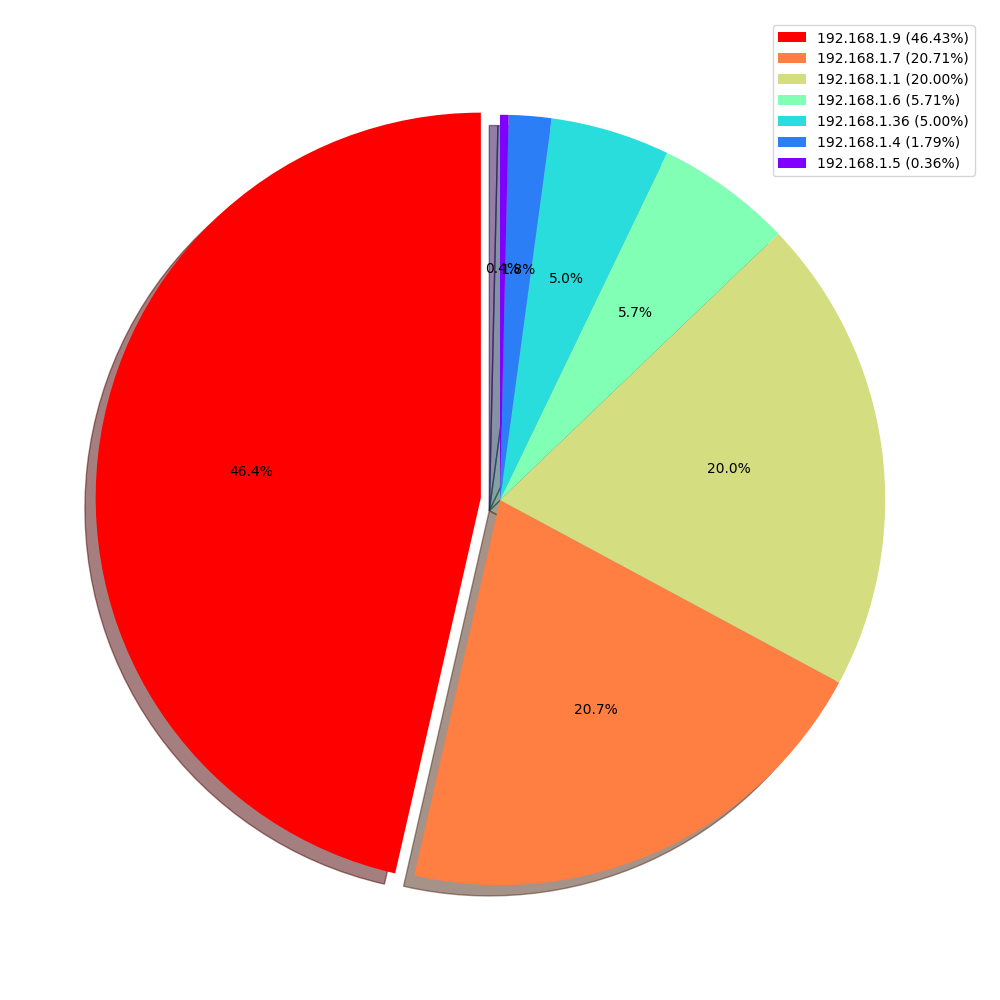
\includegraphics[width=0.45\linewidth]{../plots/mauro_s2_probabilidades.png}
		}
		\subfloat[Información de los simbolos de la fuente $S_2$ para la red de hogareña]{
		 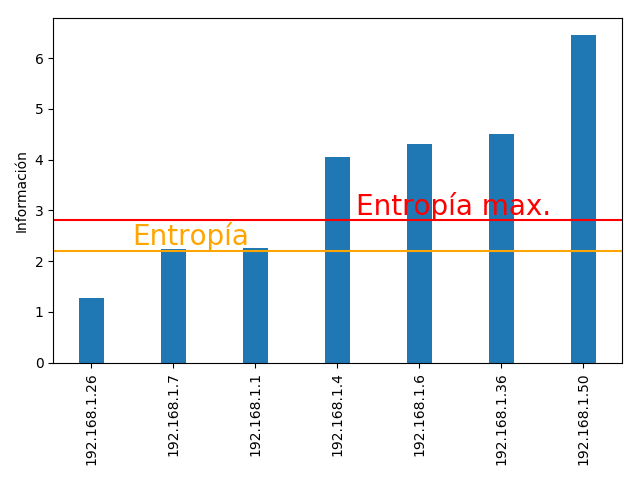
\includegraphics[width=0.55\linewidth]{../plots/mauro_s2_informacion.png}
		}
	\end{minipage}
\end{figure}

\subsubsection{Topolog\'ia de la Red}
\begin{center}
 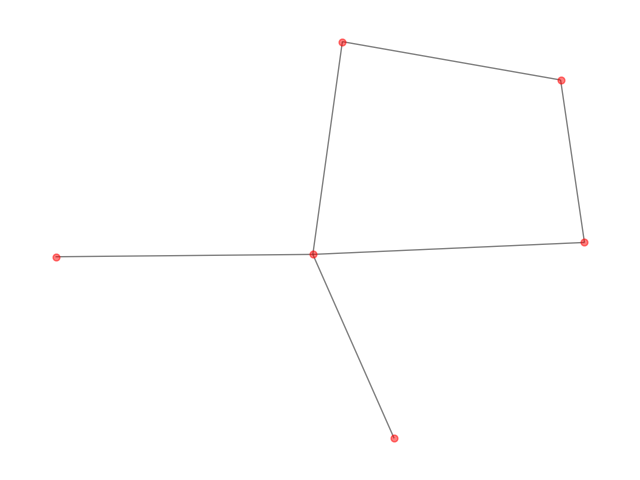
\includegraphics[scale=0.6]{../plots/mauro_s2_topologia.png}
\end{center}

\subsection{\emph{Red del Trabajo}}

En esta caso se analizo una red cableada de mediana escala, que consta de 6
oficinas con varias computadoras de escritorio (Desktop) totalizando una
cantidad de 29 estaciones. Además en cada oficina se encuentra un switch que
conecta todas las PCs de esta. La captura que se tomó fue de una hora para
poder obtener estadísticamente suficiente precision en las medidas y que estas
no sean alteradas por posibles `outliers`.

\subsubsection{Fuente Unicast-Multicast}

\begin{figure}
	\begin{minipage}[b]{0.9\linewidth}
		\subfloat[Probabilidades de los simbolos de la fuente $S_1$ para la red de oficinas]{
		 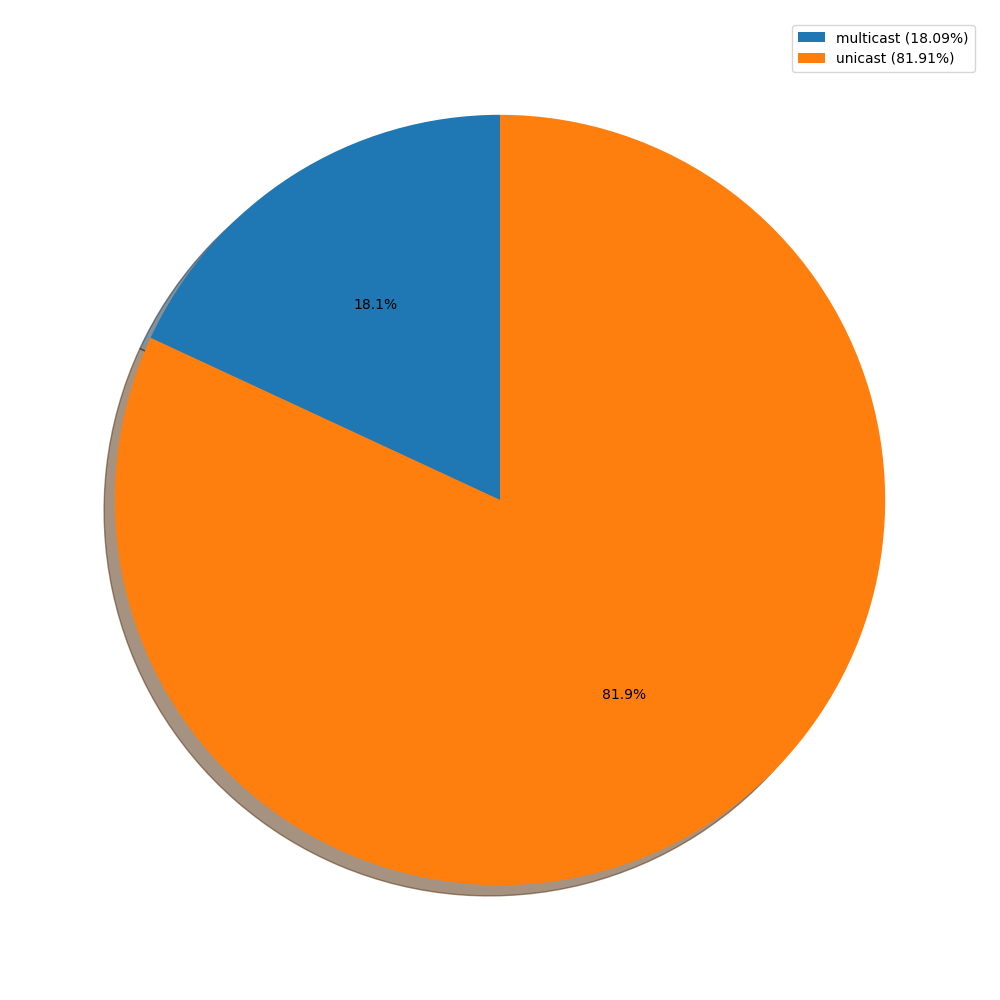
\includegraphics[width=0.45\linewidth]{../plots/trabajo_s1_probabilidades.png}
		}
		\subfloat[Información de los simbolos de la fuente $S_1$ para la red de oficinas]{
		 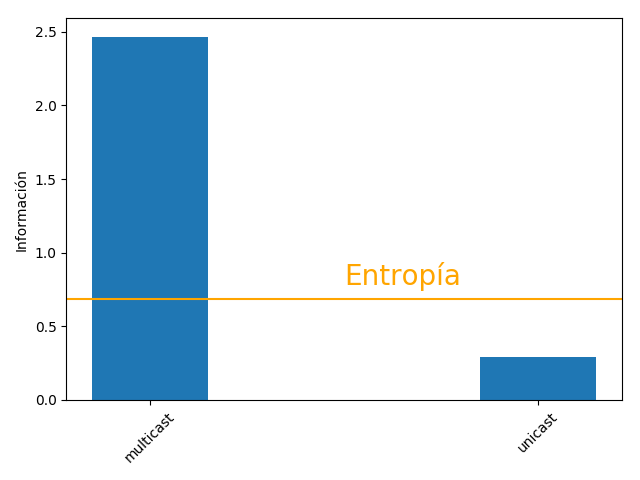
\includegraphics[width=0.55\linewidth]{../plots/trabajo_s1_informacion.png}
		}
	\end{minipage}
\end{figure}


Como se puede observar en ambos gráficos el el símbolo destacado es el
\textbf{unicast}, ya que este tiene mayor probabilidad y menor cantidad de
información. Esto nos dice que aproximadamente sobre el cable el $81.91\%$ los
paquetes fue unicast.  El sentido de esto puede deberse a que los únicos
protocolos que usan el tipo de mensajes broadcast son protocolos de control y
representan una pequeña proporción del trafico total de la red.

\clearpage

\subsubsection{Fuente ARP}

\begin{figure}
	\begin{minipage}[b]{0.9\linewidth}
		\subfloat[Probabilidades de los simbolos de la fuente $S_2$ para la red de oficinas]{
		 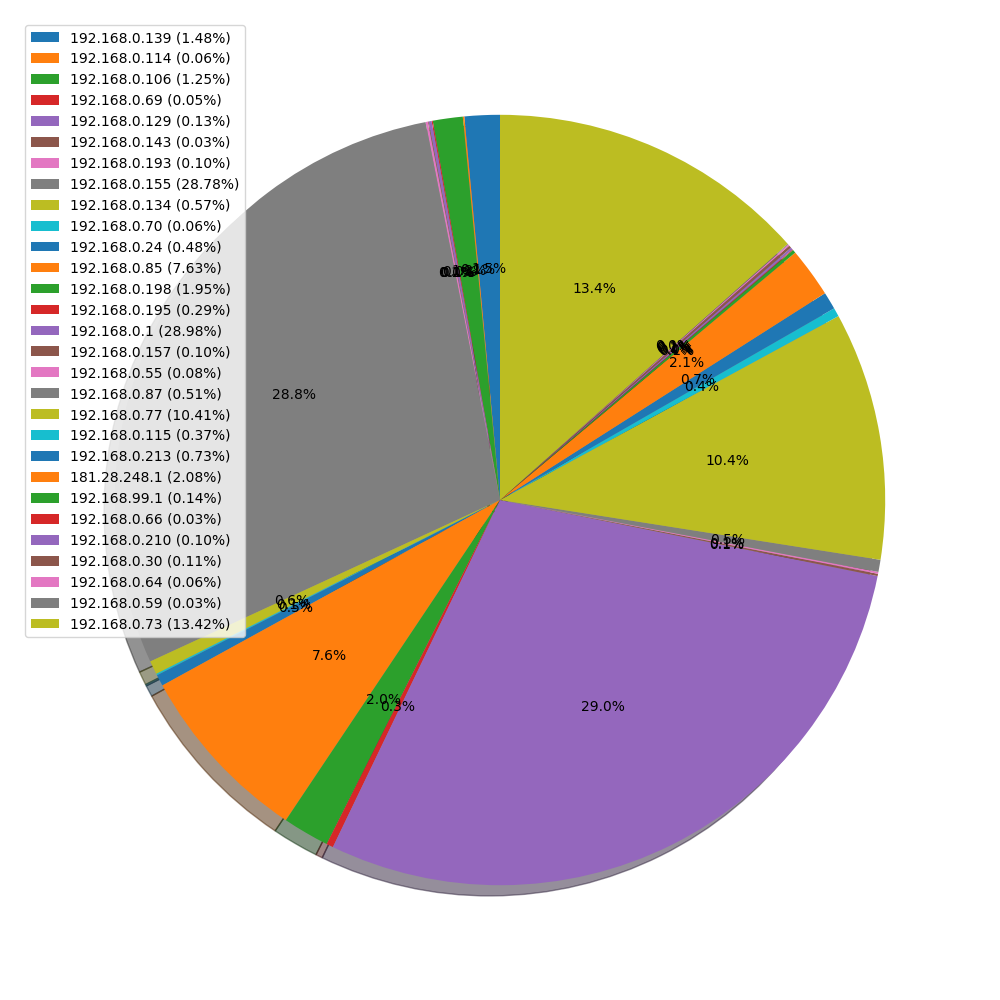
\includegraphics[width=0.45\linewidth]{../plots/trabajo_s2_probabilidades.png}
		}
		\subfloat[Información de los simbolos de la fuente $S_2$ para la red de oficinas]{
		 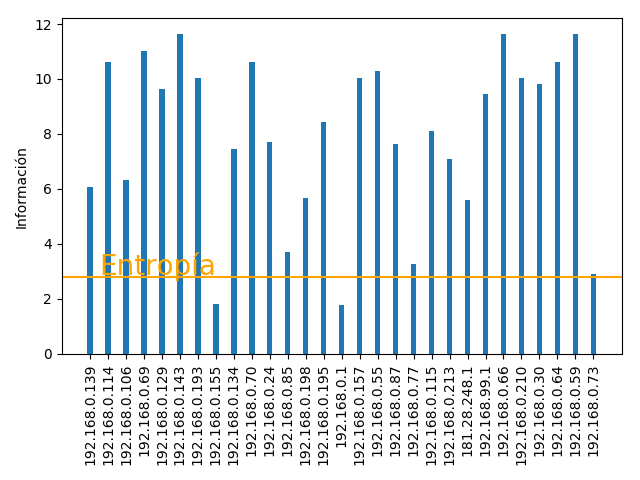
\includegraphics[width=0.55\linewidth]{../plots/trabajo_s2_informacion.png}
		}
	\end{minipage}
\end{figure}

En estos gráficos se puede ver que efectivamente el nodo \textbf{192.168.0.1}
es el destacado. Por previo conocimiento de la red se sabe que este
es el router lo cual refuerza nuestra hipótesis sobre los nodos destacados.
También se observa que la entropía alcanzada es de $2.77$ cuando la máxima
es $4.85$ y por tanto $\eta_{C} = 0.41$

\clearpage
\subsubsection{Topolog\'ia de la Red}
\begin{center}
 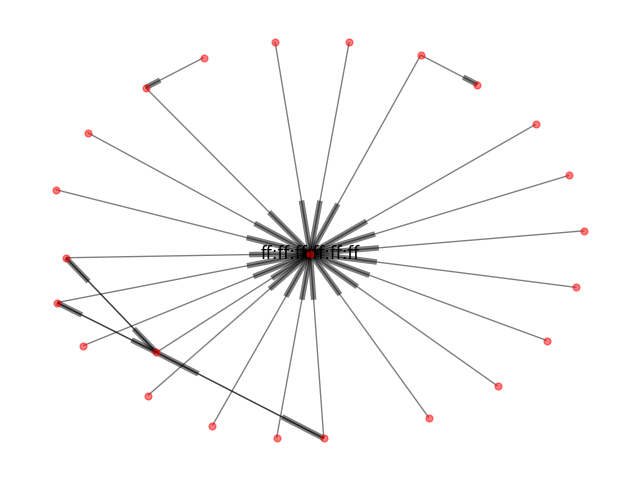
\includegraphics[scale=0.6]{../plots/trabajo_s2_topologia.png}
\end{center}

Se puede observar que la topología de mensajes arp es de tipo estrella
y que el grafo es conexo. El nodo del centro resulta ser la MAC $ff:ff:ff:ff:ff:ff$
es decir los mensajes broadcast. Se puede ver que hay pocos nodos que le hayan
enviado un paquete arp a otro que no sea el broadcast. Esto se debe
a que al estar detrás de un switch, los mensajes unicast de respuesta (\textit{is-at})
no son forwardeados a la maquina que realiza la captura aun estando en modo promiscuo
la interfaz salvo que se trate de un mensaje unicast que responde la misma maquina que
hace la captura. Aun asi se filtran mensajes unicast de pc's a otras pc's. Esto como
se dijo puede deberse a switchs que no aprendieron bien la tabla de forwardeo.

\subsection{Experimento Tavo}

\subsubsection{Fuente Unicast-Multicast}

\begin{figure}
	\begin{minipage}[b]{0.9\linewidth}
		\subfloat[Probabilidades de los simbolos de la fuente $S_1$ para la red de laboratorios]{
		 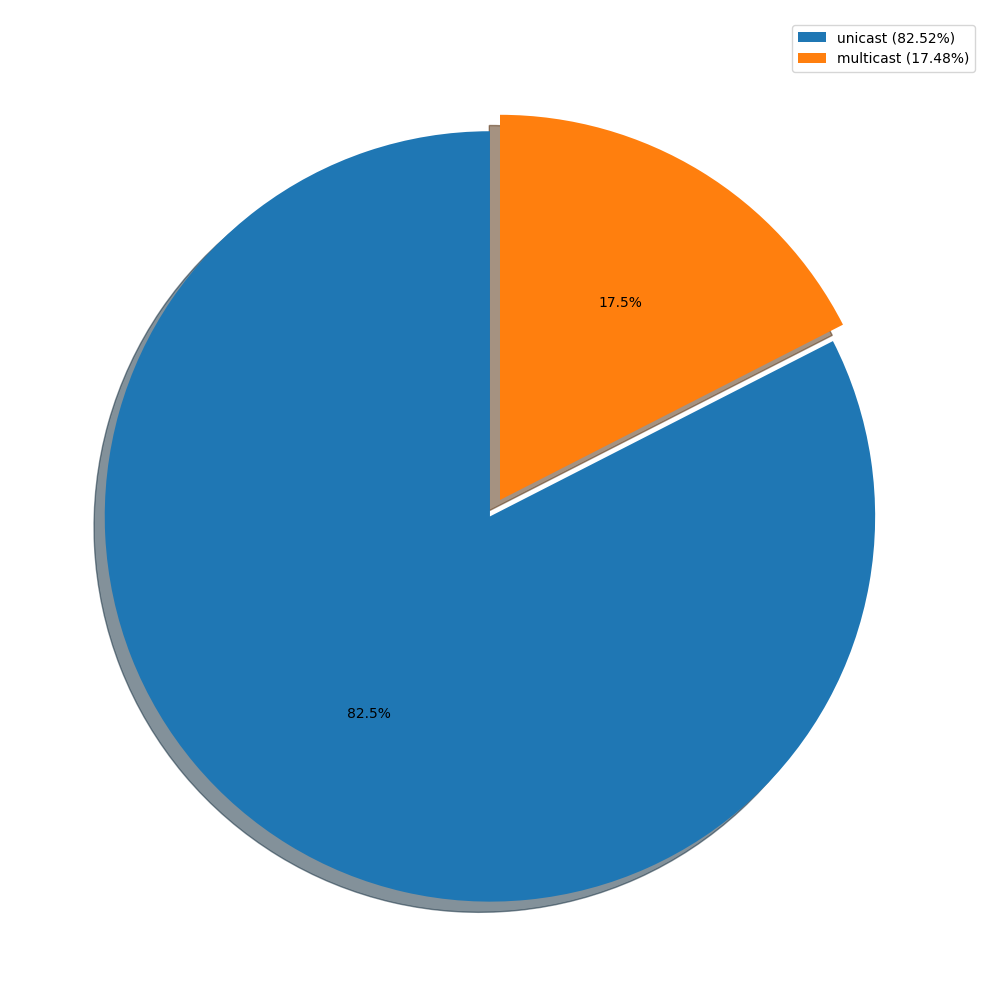
\includegraphics[width=0.45\linewidth]{../plots/labos_s1_probabilidades.png}
		}
		\subfloat[Información de los simbolos de la fuente $S_1$ para la red de laboratorios]{
		 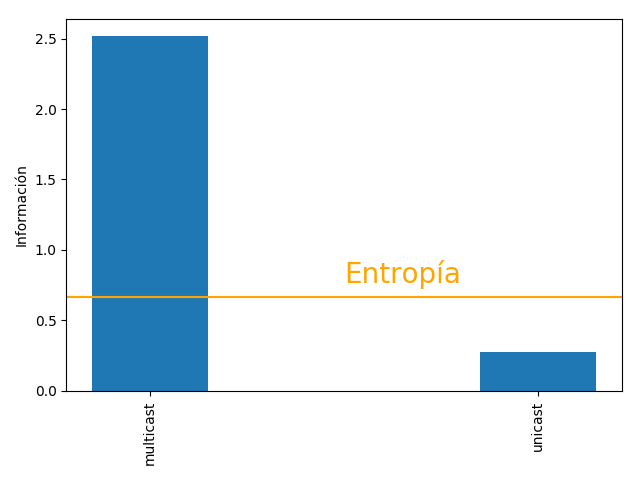
\includegraphics[width=0.55\linewidth]{../plots/labos_s1_informacion.png}
		}
	\end{minipage}
\end{figure}

\subsubsection{Fuente ARP}

\begin{figure}
	\begin{minipage}[b]{0.9\linewidth}
		\subfloat[Probabilidades de los simbolos de la fuente $S_2$ para la red de laboratorios]{
		 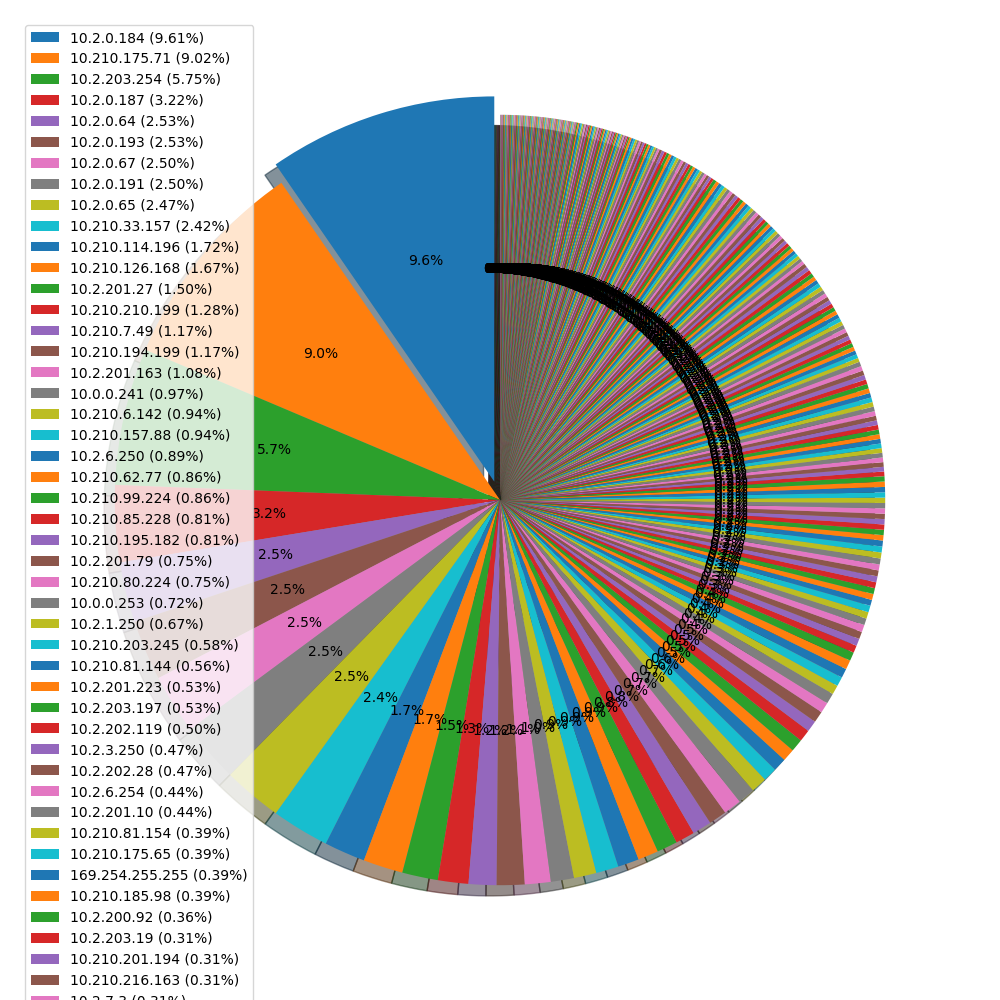
\includegraphics[width=0.45\linewidth]{../plots/labos_s2_probabilidades.png}
		}
		\subfloat[Información de los simbolos de la fuente $S_2$ para la red de laboratorios]{
		 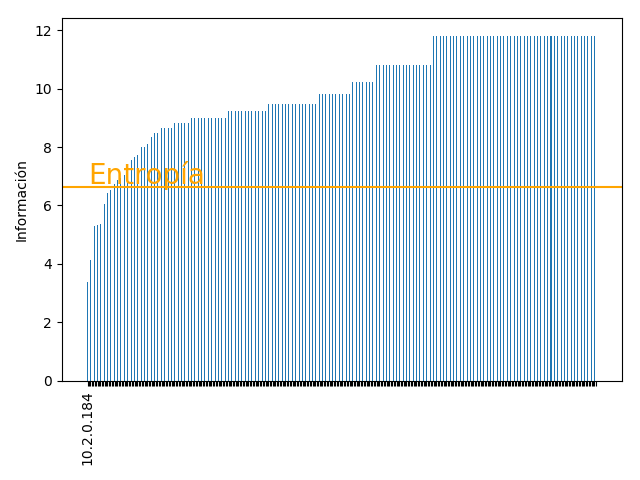
\includegraphics[width=0.55\linewidth]{../plots/labos_s2_informacion.png}
		}
	\end{minipage}
\end{figure}

\subsubsection{Topolog\'ia de la Red}
\begin{center}
 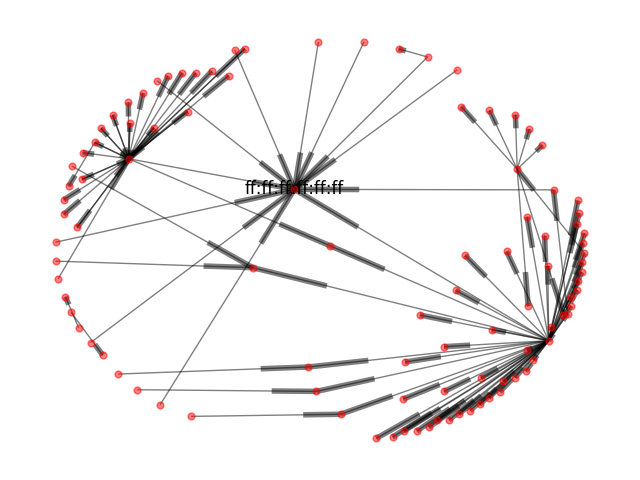
\includegraphics[scale=0.6]{../plots/labos_s2_topologia.png}
\end{center}
\begin{figure}
	\centering
	\begin{tabular}{|c|c|c|c|c|}
		\hline
		Red & Tipo & Entropía & Entropía Max & $\eta_{C}$ \\
		\hline
		Oficinas & Cableada & 2.777 & 4.858 & 0.428 \\
		\hline
		Hogareña & Wifi & 2.034 & 2.807 & 0.276 \\
		\hline
		Laboratorios & Wifi & 6.619 & 8.484 & 0.220 \\
		\hline
	\end{tabular}
	\caption[fig:tabla]{Entropía vs Max Entropía de las fuentes $S_2$ de las redes}
\end{figure}

En la figura \label{fig:tabla} se pueden ver que las redes wifi son menos compresibles ($\eta_{C}=0.276$ y $\eta_{C}=0.220$)
con respecto a la cableado ($\eta_{C}=0.428$) se puede ver en la tabla que se
reafirma nuestra hipotesis de que las redes cabledas son más compresibles que
las redes wifi.
